% !TEX root = ../main.tex

\chapter{Deep learning}
\label{ch:deep_learning}
\setlength{\marginparwidth}{3cm}\leavevmode \marginnote{\textbf{Jobin}}This chapter provides the theoretical foundation in deep learning which is required to understand the rest of the work. It starts with a historical timeline of deep learning before describing what a neural network is. Then, the notion of training a neural network, with all that is involved (like forward propagation, backpropagation, hyperparameters, data splitting or performance evaluation), is explained. This part is followed by another section devoted to a special type of neural networks, the "convolutional neural networks". They are used in many computer vision applications due to their great performance on these tasks. Finally, the concept of "transfer learning" is discussed as Chapter \ref{ch:transfer_learning} entirely relies on it.


\section{Introduction to deep learning}
\setlength{\marginparwidth}{3cm}\leavevmode \marginnote{\textbf{Jobin}}Deep learning is currently one of the trendiest topics in machine learning, a subset of artificial intelligence. Machine learning refers to statistical models that allow computers to perform specific tasks without having been explicitly programmed to solve them. In fact, these models try to find structural patterns within data in order to understand new incoming situations and react in the best possible way. There exist various techniques in machine learning such as k-NN, SVM, k-means, decision trees, association rules, etc. What mainly differentiates deep learning from these algorithms is the concept of neural networks (see Section  \ref{what_is_a_neural_network}) that are combined to form deep neural networks.

Neural networks are inspired from the biological neural networks of the brain. These systems try to learn how to solve a problem based on the data they receive as input. Many concrete applications make use of neural networks: autonomous vehicles, translators, computer-aided diagnosis systems, personal assistants, art creation, robotics, etc. The presence of deep learning techniques in these use cases clearly confirms the enthusiasm of many for this technology. Furthermore, as this field has recently gained interest (see Section \ref{historical_background}), a lot of research is still ongoing, which suggests that many exciting new applications will certainly be discovered in the near future.

\subsection{Historical background}
\label{historical_background}

\setlength{\marginparwidth}{3cm}\leavevmode \marginnote{\textbf{Jobin}}As described on Figure \ref{history}, the theoretical foundations of deep learning appeared long before the invention of computers. From the first attempts to understand the human brain until today, huge progress was made to establish the basic components of modern neural networks. One could ask why deep learning took off recently if the theory was around for a long time.

As stated by Goodfellow et al.~\cite{15}, the first part of the answer is "computing power". In fact, deep learning algorithms need a lot of data to work properly, which requires powerful CPUs/GPUs that either did not exist or were only within few people's reach. One other main reason concerns the lack of data. Since deep learning algorithms "learn" from data, learning is impossible if large amounts of good-quality data are not available. The era of Big Data enhanced deep learning possibilities. 
%%%% Je mettrais soit l'un soit l'autre. Le paragraphe du dessus c'est le paragraphe du dessous avec des autres mots :)
% These two points are summarised: "The increase in model size overtime, due to the availability of faster CPUs, the advent of general purpose GPUs, fasternetwork, connectivity and better software infrastructure for distributed computing, is one of the most important trends in the history of deep learning. This trend is generally expected to continue well into the future".\\
Finally, before the year 2012, the abilities of neural networks were still to be proven. This changed with the ImageNet Large Scale Visual Recognition Challenge (a competition where researchers evaluated their algorithms on several visual recognition tasks). In fact, the deep convolutional neural network called "AlexNet" achieved 16\% of classification error rate, whereas the previous best scores were around 25\%. This victory marked the beginning of a new craze for these types of algorithms.


\begin{figure}[!h]
\centering
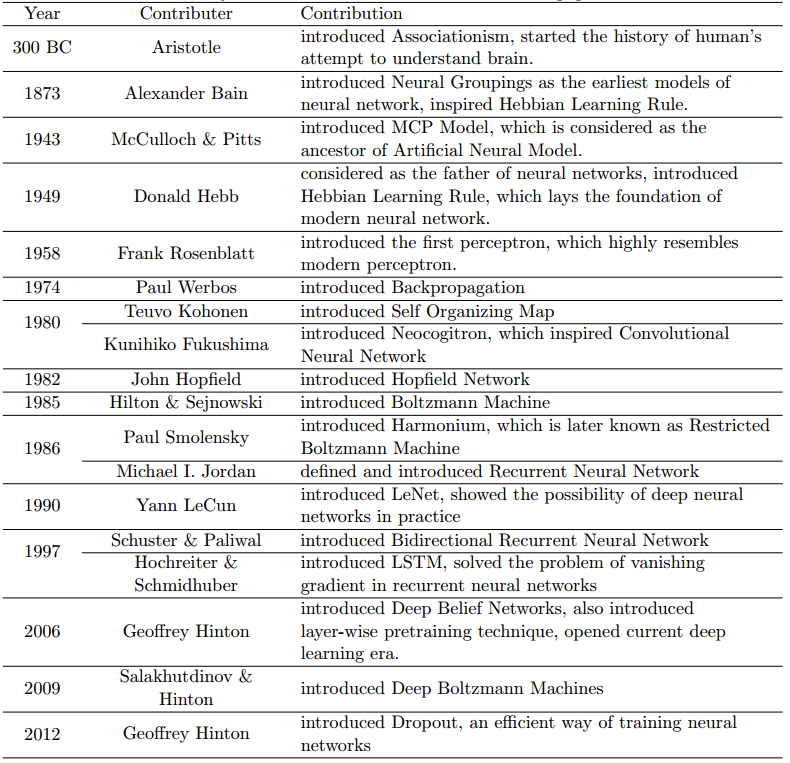
\includegraphics[width=1\textwidth, keepaspectratio=true]{./figures/history.png}
\caption{Deep learning milestones - Wang et al. \cite{14}}
\label{history}
\end{figure}

 
\subsection{What is a neural network?}
\label{what_is_a_neural_network}
\setlength{\marginparwidth}{3cm}\leavevmode \marginnote{\textbf{Jobin}}From a descriptive point of view, neural networks can simply be seen as non-linear applications that associate an input to an output with respect to certain parameters. The input can be an image, a sound or any input that can be converted into numerical features. The output of a neural network depends on the problem it tries to solve. In computer vision, the most common types of outputs are classes (for classification problems) and pixel coordinates (for segmentation problems).

\noindent From a mathematical standpoint, a neural network can be defined as a non-linear function $f$ that associates an input $x$ to an output $y$ with respect to parameters $\theta$.
\begin{equation}
y = f(x,\theta)
\end{equation}
The parameters $\theta$ are estimated from the training samples.
%\begin{figure}[!h]
%\centering
%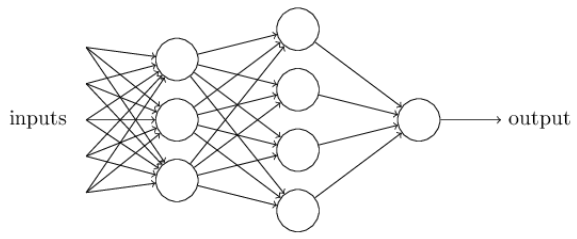
\includegraphics[width=1\textwidth, keepaspectratio=true]{./figures/neural_network.png}
%\caption{Neural Network example}
%\label{neural_network}
%\end{figure}

\subsection{Supervised and unsupervised learning}

\setlength{\marginparwidth}{3cm}\leavevmode \marginnote{\textbf{Jobin}}Machine learning algorithms can belong to two classes. The first one is "supervised learning". It includes learning algorithms whose training samples are associated with their labels in order to find the optimal mapping between the input and the output. The second one is "unsupervised learning". In contrast to supervised algorithms, the latter rely on unlabeled data. Its main goal is to infer the natural structure  present in the data. As the models presented in this work belong to the "supervised learning" category, notions explained below refer to this kind of algorithms.


\section{Neural networks basics}

\subsection{Notation}

\setlength{\marginparwidth}{3cm}\leavevmode \marginnote{\textbf{Jobin}}In order to keep the mathematical description of neural networks consistent, this work will use Andrew Y. Ng's notation~\cite{16}, who is a pioneer in deep learning.\\

\noindent \textbf{General comments}
\begin{itemize}
\item Superscript ($i)$ denotes the $i^{th}$ training example.
\item Superscript $[l]$ denotes the $l^{th}$ layer of the neural network.
\end{itemize}

\noindent \textbf{Sizes}
\begin{itemize}
\item $m$: number of examples in the dataset
\item $n_{x}$: input size
\item $n_{y}$: output size (or number of classes)
\item $n_{h}^{[l]}$: number of hidden units (i.e. neurons) of the $l^{th}$ layer
\item $L$: number of layers in the network
\end{itemize}

\noindent \textbf{Neural networks components}
\begin{itemize}
\item $X\in \R$ is the input matrix of a neural network.
\item $x^{(i)} \in \R^{n_{x}}$ is the $i^{th}$ example (sample) represented as a column vector.
\item $Y \in \R^{n_{y} \times m}$ is the label matrix.
\item $y^{(i) \in \R^{n_{y}}}$ is the output label for the $i^{th}$ example.
\item $W^{[l]} \in \R$ \textsuperscript{\# of neurons in the next layer = j  x \# of neurons in the previous layer = k} is the weight matrix at layer $[l]$.
\item $b^{[l]} \in R$\textsuperscript{\# of units in next layer} is the bias vector at the $l^{th}$ layer.
\item $\hat{y} \in R^{n_{y}}$ is the predicted output vector. It can also be denoted as $a^{[L]}$ where $L$ is the number of layers in the whole network.
\item $g^{[l]}(x)$ is the $l^{th}$ activation function.  
\item $z^{[l]} = W_{x}x^{(i)} + b^{[l]}$ denotes the weighted sum of the input given to the $l^{th}$ layer before passing through the activation function.\\
\end{itemize}

\noindent \textbf{Forward propagation equations}
\begin{itemize}
\item $a = g^{[l]}(W_{x}x^{(i)} + b^{[l]}) = g^{[l]}(z^{[l]})$ where $g^{[l]}$ denotes the $l^{th}$ layer activation function.
\item $a_{j}^{[l]} = g^{[l]} (\sum_{k} w_{jk}^{[l]}a_{k}^{[l-1]} + b_{j}^{[l]}) = g^{[l]} (z_{j}^{[l]}) $ is the general activation formula at $l^{th}$ layer.
\item $J(x, W, b, y)$ and $J(\hat{y}, y)$ denote the cost function.
\end{itemize}

\subsection{Perceptrons}
\label{perceptron}
\setlength{\marginparwidth}{3cm}\leavevmode \marginnote{\textbf{Jobin}}Perceptrons are the main components of neural networks. They were "developed in the 1950s and 1960s by the scientist Frank Rosenblatt, inspired by earlier work of Warren McCulloch and Walter Pitts"~\cite{13}. Today, they are called "artificial neurons" or simply "neurons".

The output $a$ of a perceptron $j$ is a function $f$ of input $x=(x_{1}, ..., x_{n})$ weighted by a vector of weights $w_{}=(w_{1}, ..., w_{n})$, completed by a bias $b_{j}$ and associated to a non-linear activation function $g$:
\begin{equation}
\label{perceptron_equation}
a_{j} = f_{j}(x) = g((\sum_{k=1}^{n} x_{k} * w_{k}) + b_{j})
\end{equation}
Schematically speaking, a perceptron can be represented as on Figure \ref{perceptron_model}. Each input is multiplied with its corresponding weight. The sum of these multiplications then goes through a non-linear function, called "activation function". This activation function acts like a threshold that determines the proportion of the result that goes further in the network. There exist multiple activation functions (see Section \ref{activation_functions}). It is extremely important to use non-linear functions instead of linear functions. In fact, the output of a perceptron is given as input to the others (see Section \ref{multilayer_perceptron}). Consequently, if linear functions only are used throughout the network, linear outputs are given as inputs to other linear functions. As the composition of two linear functions is itself a linear function, assembling perceptrons to create neural networks of multiple layers does not make sense in this case.


\tikzset{basic/.style={draw,fill=white!20,text width=1em,text badly centered}}
\tikzset{input/.style={basic,circle}}
\tikzset{weights/.style={basic,rectangle}}
\tikzset{functions/.style={basic,circle,fill=white!10}}



\begin{figure}[!h]
\centering
	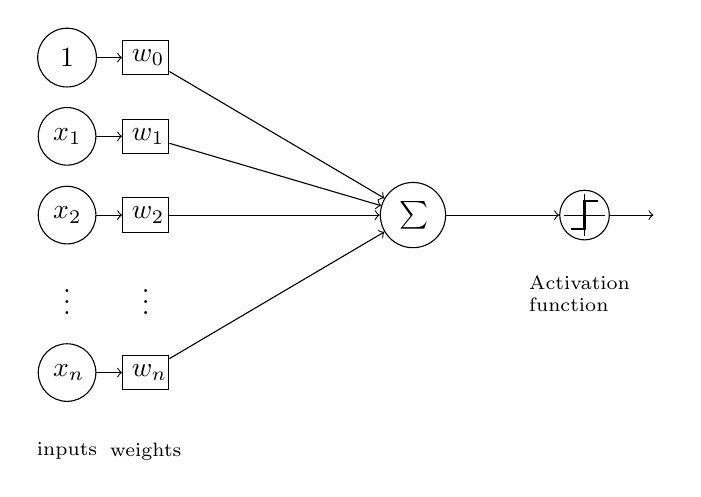
\begin{tikzpicture}
	\node[functions] (center) {};
        \node[below of=center,font=\scriptsize,text width=4em] {Activation function};
        \draw[thick] (0.5em,0.5em) -- (0,0.5em) -- (0,-0.5em) -- (-0.5em,-0.5em);
        \draw (0em,0.75em) -- (0em,-0.75em);
        \draw (0.75em,0em) -- (-0.75em,0em);
        \node[right of=center] (right) {};
            \path[draw,->] (center) -- (right);
        \node[functions,left=5em] (left) {$\sum$};
            \path[draw,->] (left) -- (center);
        \node[weights,left=15em] (2) {$w_2$} -- (2) node[input,left of=2] (l2) {$x_2$};
            \path[draw,->] (l2) -- (2);
            \path[draw,->] (2) -- (left);
        \node[below of=2] (dots) {$\vdots$} -- (dots) node[left of=dots] (ldots) {$\vdots$};
        \node[weights,below of=dots] (n) {$w_n$} -- (n) node[input,left of=n] (ln) {$x_n$};
            \path[draw,->] (ln) -- (n);
            \path[draw,->] (n) -- (left);
        \node[weights,above of=2] (1) {$w_1$} -- (1) node[input,left of=1] (l1) {$x_1$};
            \path[draw,->] (l1) -- (1);
            \path[draw,->] (1) -- (left);
        \node[weights,above of=1] (0) {$w_0$} -- (0) node[input,left of=0] (l0) {$1$};
            \path[draw,->] (l0) -- (0);
            \path[draw,->] (0) -- (left);
        \node[below of=ln,font=\scriptsize] {inputs};
        \node[below of=n,font=\scriptsize] {weights};
	
	\end{tikzpicture}
\caption{The perceptron model}
\label{perceptron_model}
\end{figure}

\subsection{Activation functions}
\label{activation_functions}
\setlength{\marginparwidth}{2cm}\leavevmode \marginnote{\textbf{Jobin}}Once the computation of the weighted sum of all inputs for a specific neuron is done, the latter has to pass the sum through an activation function. The latter must be non-linear in order to approximate extremely complex functions. In fact, neural networks are considered as universal approximators. Hornik et al. claim that "multilayer feedforward networks are capable of approximating any measurable function to any desired degree of accuracy, in a very specific and satisfying sense"~\cite{17}. According to Thomas Epelbaum~\cite{18}, the most commonly used activation functions are:\\\\
 \noindent \textbf{Sigmoid function}\\
 The sigmoid function is defined as:
 \begin{equation}
  g(x) = \frac{1}{1+e^{-x}}
 \end{equation}
 Its derivative is:
 \begin{equation}
 g'(x) = g(x)(1-g(x))
 \end{equation}
 


\begin{figure}[h!]
  \begin{center}
    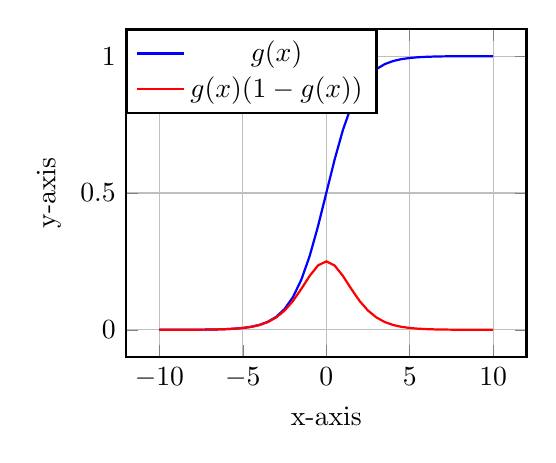
\begin{tikzpicture}
      \begin{axis}[
      	  width=0.55\linewidth, % Scale the plot to 0.7 \linewidth
          xlabel={$x$}, 
          ylabel={$y$},
          xlabel=x-axis, 
          ylabel=y-axis,
          samples=41, 
          grid, 
          thick,
          domain=-10:10,
		legend style={at={(0,1)},anchor=north west}
        ]
        \addplot+[no marks] {1/(1+exp(-x))};
        \addlegendentry{$g(x)$}
        \addplot+[no marks] {(1/(1+exp(-x))) * (1-(1/(1+exp(-x))))};
        \addlegendentry{$g(x)(1-g(x))$}
      \end{axis}
    \end{tikzpicture}
    \caption{The sigmoid function and its derivative}
  \end{center}
\end{figure} 
 
 
 \noindent \textbf{Tanh function}\\
 \begin{equation}
 g(x) = tanh(x) = \frac{1-e^{-2x}}{1+e^{-2x}}
 \end{equation}
 Its derivative is:
 \begin{equation}
 g'(x) = tanh'(x) = 1-tanh^{2}(x)
 \end{equation}
 
  \begin{figure}[h!]
  \begin{center}
    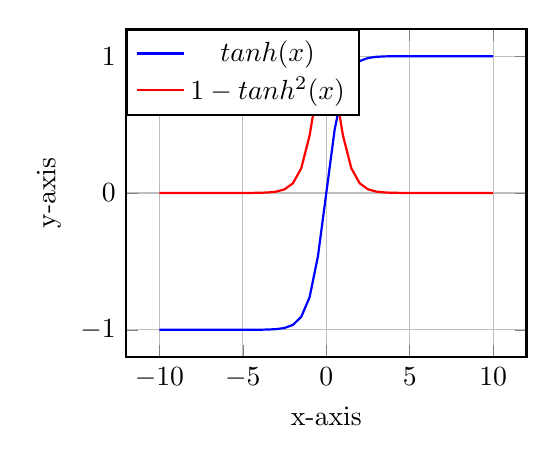
\begin{tikzpicture}
      \begin{axis}[
      	  width=0.55\linewidth, % Scale the plot to 0.7 \linewidth
          xlabel={$x$}, 
          ylabel={$y$},
          xlabel=x-axis, 
          ylabel=y-axis,
          samples=41, 
          grid, 
          thick,
          domain=-10:10,
		legend style={at={(0,1)},anchor=north west}
        ]
        \addplot+[no marks] {(1-exp(-2*x))/(1+exp(-2*x))};
        \addlegendentry{$tanh(x)$}
        \addplot+[no marks] {1-((1-exp(-2*x))/(1+exp(-2*x)))^2};
        \addlegendentry{$1-tanh^{2}(x)$}
      \end{axis}
    \end{tikzpicture}
    \caption{The tanh function and its derivative}
  \end{center}
\end{figure} 
 
 \newpage
 
 \noindent \textbf{ReLU function}\\
 \begin{equation}
 g(x) = ReLU(x) = 
 \begin{cases}
    x & \text{if } x> 0\\
    0              & \text{otherwise}
\end{cases}
 \end{equation}
 
 \begin{figure}[h!]
  \begin{center}
    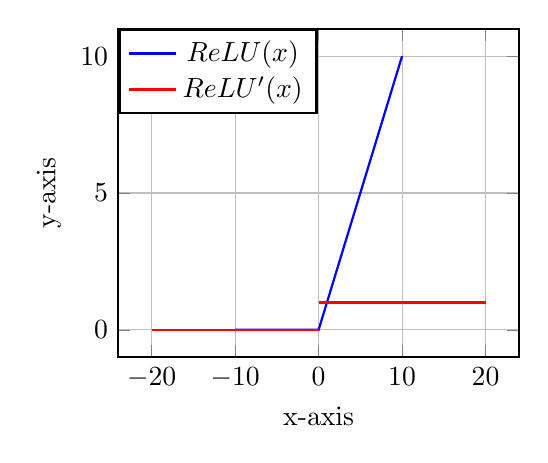
\begin{tikzpicture}[
    declare function={
    func(\x)= (\x<=0) * (0);
  }
  ]
      \begin{axis}[
      	  width=0.55\linewidth, % Scale the plot to 0.7 \linewidth
          xlabel={$x$}, 
          ylabel={$y$},
          xlabel=x-axis, 
          ylabel=y-axis,
          samples=41, 
          grid, 
          thick,
          domain=-10:10,
		legend style={at={(0,1)},anchor=north west}
        ]
        \addplot+[no marks] {(x>=0)*x};
        \addlegendentry{$ReLU(x)$}
        \addplot[domain=-20:0,red] {0};
		\addplot[domain=0:20, red] {1};
        \addlegendentry{$ReLU'(x)$}
      \end{axis}
    \end{tikzpicture}
    \caption{The ReLU function and its derivative (undefined when $x=0$)}
  \end{center}
\end{figure} 
 
 
 
 
 \noindent \textbf{ELU function}\\
 \begin{equation}
 g(x) = 
 \begin{cases}
    x & \text{if } x\geq 0\\
    e^{x}-1 & \text{otherwise }
\end{cases}
 \end{equation}
 Its derivative is:
 \begin{equation}
g'(x) = 
 \begin{cases}
    1 & \text{if } x\geq 0\\
    e^{x} & \text{otherwise }
\end{cases}
 \end{equation}
 
 

  \begin{figure}[h!]
  \begin{center}
    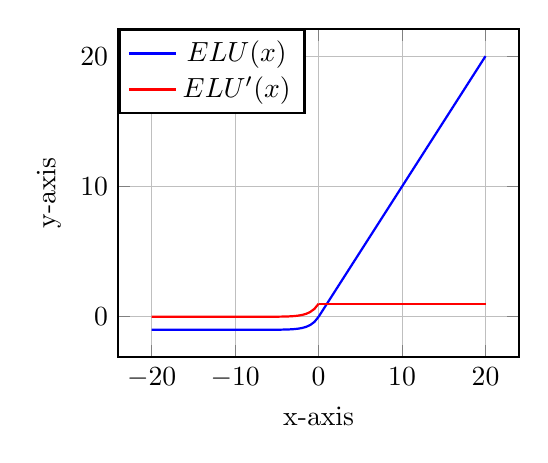
\begin{tikzpicture}[
    declare function={
    func(\x)= (\x>=0) * (x) +and (\x<0) * 4;
  }
    ]
      \begin{axis}[
      	  width=0.55\linewidth, % Scale the plot to 0.7 \linewidth
          xlabel={$x$}, 
          ylabel={$y$},
          xlabel=x-axis, 
          ylabel=y-axis,
          samples=41, 
          grid, 
          thick,
          domain=-10:10,
		legend style={at={(0,1)},anchor=north west}
        ]
        \addplot[domain=0:20, blue] {x};
        \addlegendentry{$ELU(x)$}
        \addplot[domain=0:20,red] {1};
        \addlegendentry{$ELU'(x)$}
          
        \addplot[domain=-20:0,red] {exp(x)};
        \addplot[domain=-20:0,blue] {exp(x)-1};
        
      \end{axis}
    \end{tikzpicture}
    \caption{The ELU function and its derivative}
  \end{center}
\end{figure} 

\subsection{Multilayer perceptrons}
\label{multilayer_perceptron}

\setlength{\marginparwidth}{3cm}\leavevmode \marginnote{\textbf{Jobin}}A multilayer perceptron is a type of artifical neural networks. Du et al.~\cite{23} define multilayer perceptrons as "feedforward networks with one or more layers of units between the
input and output layers" where "the output units represent a hyperplane in the space
of the input patterns". A multilayer perceptron is composed of $L$ layers, each of them composed of $n^{l}_{h}$ perceptrons. The layers are organized in the following way:
\begin{itemize}
\item The input layer: It is the neural network entry point for the data. Generally speaking, the data are provided in the form of a matrix $X \in \R$ of size $(n_{x} \times batch\_size)$ with their corresponding labels $Y \in \R$ of size $(n_{y} \times batch\_size)$. The batch size defines the number of samples that will be fed to the network at the same time and $n_{x}$ is the dimension of each sample. Moreover, $x^{(i)}$ is the $i^{th}$ sample represented as a column vector. The total number of training samples is given by $m$. Finally, $y^{(i)}$ is the output label for the $i^{th}$ example. For instance, suppose the number of samples is 100 and the batch size 32. In this situation, the network will be fed with 4 batches of sizes [32, 32, 32, 4] respectively. 

\item The hidden layer(s): Hidden layers stand for all layers that are between the input layer and the output layer. Each of them has its own weights and biases (W, b), denoted by $W^{[l]} \in \R $ and $b^{[l]}$ respectively, where $W_{ij}^{l}$ corresponds to the weights associated with the connection between perceptron $j$ in \mbox{layer $l$} and perceptron $i$ in layer $l+1$. By analogy, $b_{i}^{[l]}$ is the bias associated with perceptron $i$ in layer $l$. Weights and biases are the parameters to optimize in order to obtain the best mapping between the input and the output of the network (see Section \ref{training_a_neural_network}). Before training the neural network, the weights can be randomly initialized or initialized with more sophisticated methods such as "Xavier initialization" or "Kaiming initialization" (see Section \ref{weight_initialization}).

\item The output layer: It is the last layer of the neural network. Its role is essential since it produces the prediction of the network for a given input. The prediction of a neural network is given by $\hat{y} \in R^{n_{y}}$ with $n_{y}$ representing the number of different labels. In a classification task, whose goal is to assign a specific class to each input, $\hat{y}$ is usually the probability that the input belongs to each class. In this case, the \textit{softmax} activation function would be used at the end.
\end{itemize}
The advantage of organizing the weights, biases and inputs in matrices is due to the ability of modern CPUs/GPUs to quickly perform linear algebra computations. This way of structuring the network components is called "vectorization" which avoids using loops in the code, which would considerably slow down the computations.
Figure \ref{multilayer_perceptrons_figure} illustrates the concept of multilayer perceptrons. In this example, the total number of layers $L$ is equal to 3, the input size $n_{x}$ is equal to 4 and the number of units of each layer is $n_{h}^{1}= 4$, $n_{h}^{2}=2$, $n_{h}^{3}=1$. The network contains the weights  $W^{(1)} \in \R^{2x3}$, $W^{(2)} \in \R^{1x2}$ and the biases  $b^{[1]} \in \R^2$, $b^{[2]} \in \R^1$.


\begin{figure}[!h]
\centering
	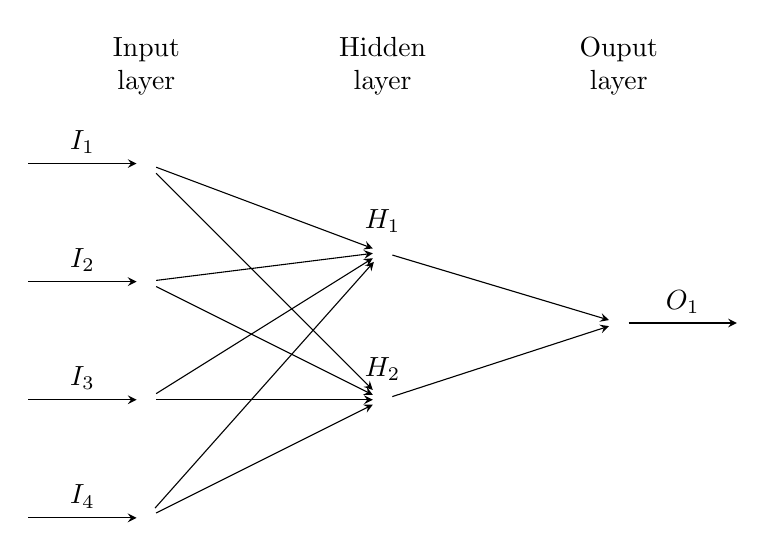
\begin{tikzpicture}[x=1.5cm, y=1.5cm, >=stealth]
	
	\foreach \m/\l [count=\y] in {1,2,3,4}
	  \node [every neuron/.try, neuron \m/.try] (input-\m) at (0,2.5-\y) {};
	
	\foreach \m [count=\y] in {1,2}
	  \node [every neuron/.try, neuron \m/.try ] (hidden-\m) at (2,2-\y*1.25) {};
	
	\foreach \m [count=\y] in {1}
	  \node [every neuron/.try, neuron \m/.try ] (output-\m) at (4,0.15) {};
	
	% input layer
	\foreach \l [count=\i] in {1,2,3,4}
	  \draw [<-] (input-\i) -- ++(-1,0)
	    node [above, midway] {$I_\l$};
	
	% hidden layer
	\foreach \l [count=\i] in {1,2}
	  \node [above] at (hidden-\i.north) {$H_\l$};
	
	% output neurons
	\foreach \l [count=\i] in {1}
	  \draw [->] (output-\i) -- ++(1,0)
	    node [above, midway] {$O_\l$};
	
	% input -> hidden
	\foreach \i in {1,...,4}
	  \foreach \j in {1,...,2}
	    \draw [->] (input-\i) -- (hidden-\j);
	
	% hidden -> output
	\foreach \i in {1,...,2}
	  \foreach \j in {1}
	    \draw [->] (hidden-\i) -- (output-\j);
	
	% labels above layers
	\foreach \l [count=\x from 0] in {Input, Hidden, Ouput}
	  \node [align=center, above] at (\x*2,2) {\l \\ layer};
	
	\end{tikzpicture}
\caption{Multilayer perceptrons}
\label{multilayer_perceptrons_figure}
\end{figure}

\section{Training a neural network}
\label{training_a_neural_network}

\setlength{\marginparwidth}{3cm}\leavevmode \marginnote{\textbf{Jobin}}Training a neural network can be broken down into multiple steps. The first one is the "forward propagation" step. It consists in giving examples that need to be classified (or segmented, depending on the task) to the untrained neural network and to spread intermediate results through all layers of the network. %Passing all batches as input to a network is called an "epoch". 
After seeing every single batch, the loss is computed using a "loss function". The latter is used to evaluate the predictions of the neural network in comparison to their ground truth. Then, the weights and biases of the network are updated during a process called "backpropagation" in order to find the global minimum of the loss function. As soon as the neural network has seen every single batch, the end of an "epoch" is reached. This process is repeated for a defined number of epochs.


\subsection{Forward propagation}

\setlength{\marginparwidth}{3cm}\leavevmode \marginnote{\textbf{Jobin}}The forward propagation is used to transmit the input through the entire neural network. Mathematically speaking, the forward propagation step for a specific \mbox{layer $l$} is represented by two equations. The first equation denotes the weighted sum of the input given to the $l^{th}$ layer before passing through the activation function $g$: 
\begin{equation}
z^{[l]} = W_{x}^{[l]}x^{(i)} + b^{[l]}
\end{equation}
The second equation describes the effect of the activation function:
\begin{equation}
a^{[l]} = g^{[l]}(z^{[l]})
\end{equation}
Since the output of the activation function is then given as input to all the neurons of the next layer, the whole forward propagation step can be defined as:
\begin{equation}
a_{j}^{[l]} = g^{[l]} (\sum_{k} w_{jk}^{[l]}a_{k}^{[l-1]} + b_{j}^{[l]}) = g^{[l]} (z_{j}^{[l]}) 
\end{equation}
Figure \ref{forward_propagation} illustrates the computation of the forward propagation pass for the $l^{th}$ layer. The weight matrix $W_{jk}^{l}$ represents the weights associated with the connection between perceptron $k$ in layer $l$ and perceptron $j$ in layer $l+1$. This matrix is multiplied by the output of the previous layer $a_{j}^{[l-1]}$ before adding the bias $b^{[l]}$. The result is given as input to the activation function.

\begin{figure}[!h]
\centering
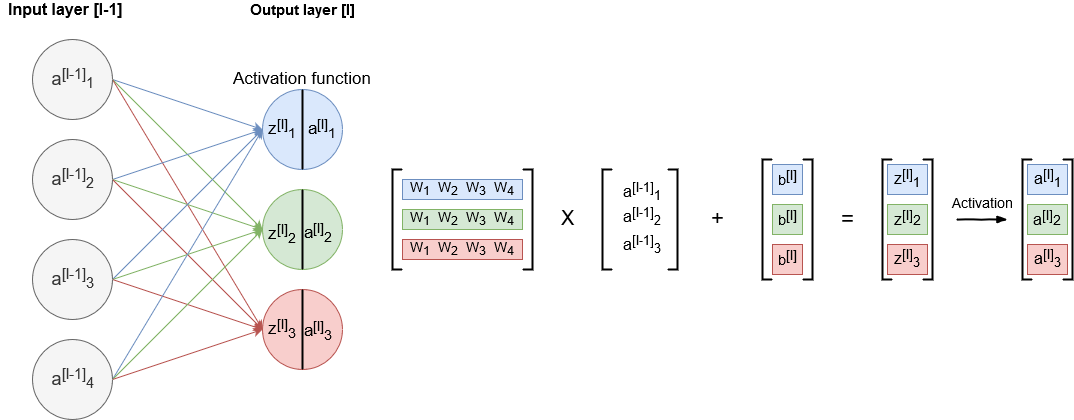
\includegraphics[width=1\textwidth, keepaspectratio=true]{./figures/forward_propagation.png}
\caption{Forward propagation }
\label{forward_propagation}
\end{figure}

\subsection{Loss computation}

\setlength{\marginparwidth}{3cm}\leavevmode \marginnote{\textbf{Jobin}}As stated by Thomas Epelbaum, "the loss function evaluates the error performed by the neural network when it tries to estimate the data to be predicted"~\cite{18}. It is therefore useful to measure the penalty for a single input. On the contrary, when the goal is to get a more general overview of the error on the entire batch or on the entire dataset, the cost function $J$ is used. The latter is represented by $J(\hat{y}, y)$ where $\hat{y}$ is the prediction of the neural network and $y$ the real label. There exist multiple cost functions.\\
For a regression problem, a commonly used loss function is the mean squared error:
\begin{equation}
J(\hat{y}, y) = \frac{1}{m}[\sum_{i=1}^{m} (\hat{y}^{(i)} - y^{(i)})^{2}]
\end{equation}
For classification problems, the cross entropy function is regularly used. The binary classification where the number of classes $n_{y}$ = 2 is distinguished from the multiclass classification where $n_{y}$ > 2. In the case of binary classification, the cross entropy is:
\begin{equation}
J(\hat{y}, y) = -\frac{1}{m}\sum_{i=1}^{m} [y_{i}*log(\hat{y}_{i}) + (1-y_{i})*log(1-\hat{y_i})]
\end{equation}
In the case of multiclass classification, the categorical crossentropy is given by:
\begin{equation}
J(\hat{y}, y) = - \sum_{i=1}^{n_{y}} \sum_{j=1}^{m} (y_{ij}*log(\hat{y}_{ij}))
\end{equation}
As the cost function gives an estimation of the overall error of the network, the main objective of training a neural network is to update its weights in order to approach the minimum of the function. Therefore, deep learning problems can be considered as optimization problems. Solutions to these problems can be found using the gradient descent algorithm during backpropagation.

\subsection{Backpropagation}

\setlength{\marginparwidth}{3cm}\leavevmode \marginnote{\textbf{Jobin}}Backpropagation relies on a technique called "gradient descent" to minimize the cost function $J(W, b)$. Generally speaking, "the intuition behind the backpropagation algorithm is as follows. Given a training example $(x^{(i)}, y^{(i)})$, we will first run a forward pass to compute all the activations throughout the network, including the output value of the network. Then, for each node $i$ in layer $l$, we would like to compute an "error term" $\partial^{(l)}_{i}$ that measures how much that node was "responsible" for any errors in our output. For an output node, we can directly measure the difference between the network’s activation and the true target value, and use that to define $\partial^{(n_{l})}_{i}$(where layer $n_{l}$ is the output layer). How about hidden units? For those, we will compute $\delta^{(l)}_{i}$ based on a weighted average of the error terms of the nodes that uses $a^{(l)}_{i}$ as an input"~\cite{24}.

In other words, after each forward pass through the entire network, backpropagation performs a backward pass which aims at minimizing the cost function by adjusting the parameters of the model. The way parameters are updated is defined by the gradients of the cost function with respect to each parameter of the network. The gradient of the cost function $J(x_{1}, x_{2}, ..., x_{m})$ at point $x$ is given by:
\begin{equation}
\frac{\partial J}{\partial x} = [\frac{\partial J}{\partial x_{1}}, \frac{\partial J}{\partial x_{2}}, ..., \frac{\partial J}{\partial x_{m}}]
\end{equation}
The gradient shows how much the parameters that constitute $x$ need to change to minimize the function. In neural networks, the parameters of the cost function are all weight matrices $W^{[l]}$ and biases $b^{[l]}$. The computation of all these gradients relies on the "chain rule". In the case of weights, the chain rule is:
\begin{equation}
\frac{\partial J}{\partial w_{jk}^{l}} = \frac{\partial J}{\partial z_{j}^{l}} * \frac{\partial z_{j}^{l}}{\partial w_{jk}^{l}}
\end{equation}
Similarly, the chain rules has to be applied to the biases:
\begin{equation}
\frac{\partial J}{\partial b_{j}^{l}} = \frac{\partial J}{\partial z_{j}^{l}} * \frac{\partial z_{j}^{l}}{\partial b_{j}^{l}}
\end{equation}
Once the gradients of each parameter are computed, the corresponding parameters are updated. The weight update is described by the following equation:
\begin{equation}
W^{[l]} = W^{[l]} - \alpha * \frac{\partial J}{\partial W^{[l]}}
\end{equation}
The bias update corresponds to:
\begin{equation}
b^{[l]} = b^{[l]} - \alpha * \frac{\partial J}{\partial b^{[l]}}
\end{equation}
%The hyperparameter $\alpha$ of these two equations is called "learning rate". It determines the gradient's influence at each epoch and has to be manually tuned.
The "learning rate" $\alpha$ determines the influence that the gradient has at each epoch. It is an hyperparameter and has to be manually tuned.


\subsection{Metrics}

\setlength{\marginparwidth}{3cm}\leavevmode \marginnote{\textbf{Jobin}}In classification tasks, four separate output labels can occur:
\begin{itemize}
\item True Positive (TP):  an output belongs to this class if the prediction that the latter \textbf{contains} a certain feature is \textbf{correct}.
\item True Negative (TN): an output belongs to this class if the prediction that the latter does \textbf{not contain} a certain feature is \textbf{correct}.
\item False Positive (FP): an output belongs to this class if the prediction that the latter \textbf{contains} a certain feature is \textbf{incorrect}.
\item False Negative (FN): an output belongs to this class if the prediction that the latter does \textbf{not contain} a certain feature is \textbf{incorrect}.
\end{itemize}
From these four categories, multiple metrics with their own specificities can be computed~\cite{25}:
\begin{itemize}
\item Accuracy: "Ratio of the correctly labeled subjects to the whole pool of subjects".
\begin{equation}
Accuracy = \frac{(TP+TN)}{TP+FP+FN+TN}
\end{equation}
Accuracy is a great measure in the case of symmetric data (i.e. the number of FN $\approx$ FP and their cost is similar). When this condition is not fulfilled, accuracy can lead to bad models. For instance, suppose that a binary classification model always outputs class 0. If the data is composed of 99 samples from class 0 and 1 sample from class 1, the accuracy is equal to 99\%, but the model is not smart. Consequently, this metric has to be used in addition to other metrics.

\item Precision: "Ratio of the correctly labeled positive subjects to all positively labeled subjects"
\begin{equation}
Precision = \frac{TP}{(TP + FP)}
\end{equation}
This metric is recommended when the confidence of the true positives predicted by the model is important. For instance, this happens in the case of spam blockers where it is preferable to have a spam in the mailbox rather than a regular mail in the spam folder.

\item Recall (sensitivity): "Ratio of the correctly labeled positive subjects to all subjects whose class is actually positive".

\begin{equation}
Recall = \frac{TP}{(TP + FN)}
\end{equation}
This metric is recommended when the occurence of false negatives is intolerable and false positives are preferred. This makes perfect sense for disease detection models: labeling an healthy person as unhealthy is better than labeling an unhealthy person as healthy.

\item F1-score: Harmonic mean (average) of the precision and recall.
\begin{equation}
F1\operatorname{-}score = \frac{2* recall * precision}{(recall + precision)}
\end{equation}
F1-score considers both precision and recall and is the highest if these two metrics are balanced. This metric is perfectly suitable when the cost of false positives and false negatives is not the same.

\item Specificity: "Ratio of the correctly labeled negative subjects to all subjects whose class is actually negative."
\begin{equation}
Specificity = \frac{TN}{(TN + FP)}
\end{equation}
This metric is recommended when the occurence of false positives is intolerable whereas true negatives are desired. For instance drug tests can not indicate false positives but they have to cover all true negatives.

\item ROC curve and AUC:
As explained by Sarang Narkhede~\cite{26}, "the ROC curve is plotted with the true positive rate (=recall) against the false positive rate (1-specificity) where recall is on y-axis and the false positive rate is on the x-axis. AUC-ROC curve is a performance measurement for classification problem at various thresholds settings. ROC is a probability curve and AUC represents degree or measure of separability. It tells how much model is capable of distinguishing between classes. Higher the AUC, better the model is at predicting 0s as 0s and 1s as 1s".

\end{itemize}




\subsection{Data}

\setlength{\marginparwidth}{3cm}\leavevmode \marginnote{\textbf{Jobin}}In deep learning, data is essential. As seen previously, neural networks learn features from it. Therefore, data has to be handled carefully and in the right way. Usually, it is split into three different sets:
\begin{itemize}
\item The training set: This is the part of the dataset that is used to train the neural network (the weights and biases).
\item The validation set: This dataset is used to evaluate a trained model. Usually, the evaluation on the validation set is performed every $N$ epochs, where $N$ is a fixed number. The validation set needs to come from the same distribution as the training set but should exclusively contain unseen data. This last point is crucial since the validation set shows how well the neural network generalizes on unknown data. The validation set can also be used as an indicator to decide when the training should be stopped in order to prevent "overfitting" which is the behaviour of a model that fits to the training set too closely and do not generalize well. In fact, if the validation loss continuously increases for a certain number of epochs, going on with the training will increase the overfit. The fact of interrupting the training earlier is called "early stopping".
\item The test set: This last part of the dataset is used to establish the final evaluation of the model. It also contains unseen data exclusively. 
\end{itemize}
The way these three sets are split mostly depends on the number of samples available. If the latter is big, the data is split into training and test sets using the ratio 80/20. Then, the remaining training samples are also split into training and validation using the ratio 80/20. On the contrary, if there are few data available, k-fold cross-validation is a good practice. This technique consists in splitting the entire dataset into k folds. One fold is picked as test set and the others are considered as training sets. The model is trained on training folds and tested on the test fold. Then, another test set is picked and the same process is repeated until all possible test sets are picked. At the end of the process, the results of all test sets are averaged, which provides a good estimation of the model's performance. This technique is summarized on Figure \ref{cross_validation}.

\begin{figure}[!h]
\centering
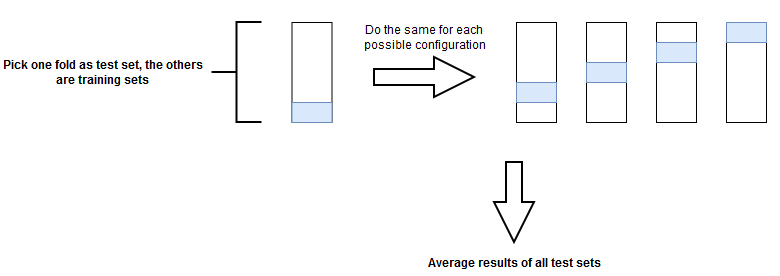
\includegraphics[width=1\textwidth, keepaspectratio=true]{./figures/cross_validation.png}
\caption{5-fold cross-validation}
\label{cross_validation}
\end{figure}


\subsection{Weight initialization}
\label{weight_initialization}
\setlength{\marginparwidth}{3cm}\leavevmode \marginnote{\textbf{Jobin}}Before training a neural network, the weights have to be initialized in order to proceed to the first forward propagation. The initialization of the neural network weights is crucial since it will determine how quickly the network converges to an optimum. According to James Dellinger, the idea behind weight initialization is to generate an initialization that "prevents layer activation outputs from exploding or vanishing during the course of a forward pass through a deep neural network. If either occurs, loss gradients will either be too large or too small to flow backwards beneficially, and the network will take longer to converge, if it is even able to do so at all"~\cite{27}.

The simplest and least efficient technique to initialize neural network weights is to randomly generate them. The major problem of this technique comes from the fact that some initializations can lead to extremely small or big values that lead to values near 0 or 1 for most activation functions. Consequently, the slope of the gradient changes slowly and the learning process takes a lot of time.\\
To prevent this effect when the tanh activation function is used, "Xavier initialization" multiplies the random initialization by the fraction:
\begin{equation}
\frac{\sqrt{6}}{\sqrt{n_{h}^{[l]}+n_{h}^{[l+1]}}}
\end{equation}
where $n_{h}^{[l]}$ is the number of incoming network connections to the layer and $n_{h}^{[l+1]}$ is the number of outgoing network connections from that layer.\\
For activation functions that are not symmetric around zero and do not have outputs inside the range $[-1,1]$ such as ReLU or ELU, Kaiming initialization is an alternative. It consists in multiplying the randomly initialized weight matrix by:
\begin{equation}
\frac{\sqrt{2}}{\sqrt{n_{h}^{[l]}}}
\end{equation} 
where $n_{h}^{[l]}$ is the number of incoming connections coming to a given layer from the previous layer's output.

\subsection{Hyperparameter tuning}

\setlength{\marginparwidth}{3cm}\leavevmode \marginnote{\textbf{Jobin}}Hyperparameters denote parameters that cannot be directly learned from the data. That is the case for the learning rate, the batch size and the number of epochs that were described in previous sections. So, these parameters have to be manually tuned in order to find the best configuration (i.e. the one that minimizes the cost function and that keeps an acceptable level of generalization).

Regarding the learning rate $\alpha$, its value has to be neither too large nor too small. A too large learning rate is recognizable by analyzing the training loss curve: if the loss is exploding, oscillating or if there is no improvement and it is stuck around a suboptimal local optima, the learning rate is too high and should be decreased. On the contrary, if the learning is very slow and the loss does not decrease, or if the model is overfitting, it is a clear sign that it should be increased. The learning rate can take a wide range of values. Consequently, the most used technique to find the optimal learning rate is simply the "trial and error" method, which consists in "trying widely different learning rates to determine the range of learning rates that need to be explored"~\cite{28}. There also exist methods that, instead of keeping a fixed learning rate for the entire training, reduce it after each epoch (learning rate decay) or each time the loss on the validation set does not decrease (learning rate scheduling).

Batch size is another important hyperparameter to tune. Training a network with a small batch size "requires less memory, since the latter is trained using fewer samples"~\cite{29}. Furthermore, "networks train faster because the weight update is done after each propagation" \cite{29}. Nevertheless, "the smaller the batch, the less accurate the estimate of the gradient will be"~\cite{29}. Indeed, due to the high weight update frequency, the gradient fluctuates much more than if it was computed after a bigger number of samples.

Finally, the number of epochs during which the network is trained has to be carefully chosen. In fact, from a certain point in the training onwards, neural networks do not learn anymore useful features in the data and start overfitting. This point corresponds to the moment where the validation loss does not decrease anymore and starts increasing continuously. It is at this moment that the training should stop. To achieve this goal, it is either possible to directly choose the right number of epochs or to use the so-called "early stopping" method which stops the training as soon as the validation loss does not decrease for $N$ epochs.


\section{Convolutional Neural Networks}

\setlength{\marginparwidth}{3cm}\leavevmode \marginnote{\textbf{Cl{\'e}ment}}Convolutional Neural Networks (CNN) are a specific type of deep neural networks. They are particular in that they contain layers which perform a mathematical operation named "convolution" on the input data. CNNs are mostly used in image and video analysis.

To perform a convolution, numerical input data and a "filter" are required. A filter can be seen as an $f*f$ numerical patch that moves across the entire input. It first moves horizontally until reaching the right-most border of the image. Then, it goes down a cell and starts from the border on the left-hand side. This process is repeated until the filter reaches the bottom-right corner of the image, which marks the end of the convolution. At each step, the dot product between the filter and the part of the input covered by the filter is computed. Figure \ref{fig:convolution} showcases a simple convolution which aims at finding vertical lines in a black and white image. For example, the output of the first step of the convolution (in red) is computed by evaluating the dot product between the blue filter and the red part of the input image: 
\begin{equation}
\begin{gathered}
\color{blue}(-1) \color{black}* \color{red}0 \color{black}+ \color{blue}2 \color{black}* \color{red}0 \color{black}+ \color{blue}(-1) \color{black}* \color{red}0
\\ \color{black}+ \\ 
\color{blue}(-1) \color{black}* \color{red}0 \color{black}+ \color{blue}2 \color{black}* \color{red}0 \color{black}+ \color{blue}(-1) \color{black}* \color{red}1 
\\ \color{black}+ \\ 
\color{blue}(-1) \color{black}* \color{red}0 \color{black}+ \color{blue}2 \color{black}* \color{red}0 \color{black}+ \color{blue}(-1) \color{black}* \color{red}1 
\\ \color{black}= -2
\end{gathered}
\end{equation}

\noindent The output of the entire convolution shows negative values in the outside parts and large positive values in the center. This means that the $3*3$ filter detected a vertical line in the center of the input image. Like other parameters, filters are learned while training. 

\begin{figure}[!h]
\centering
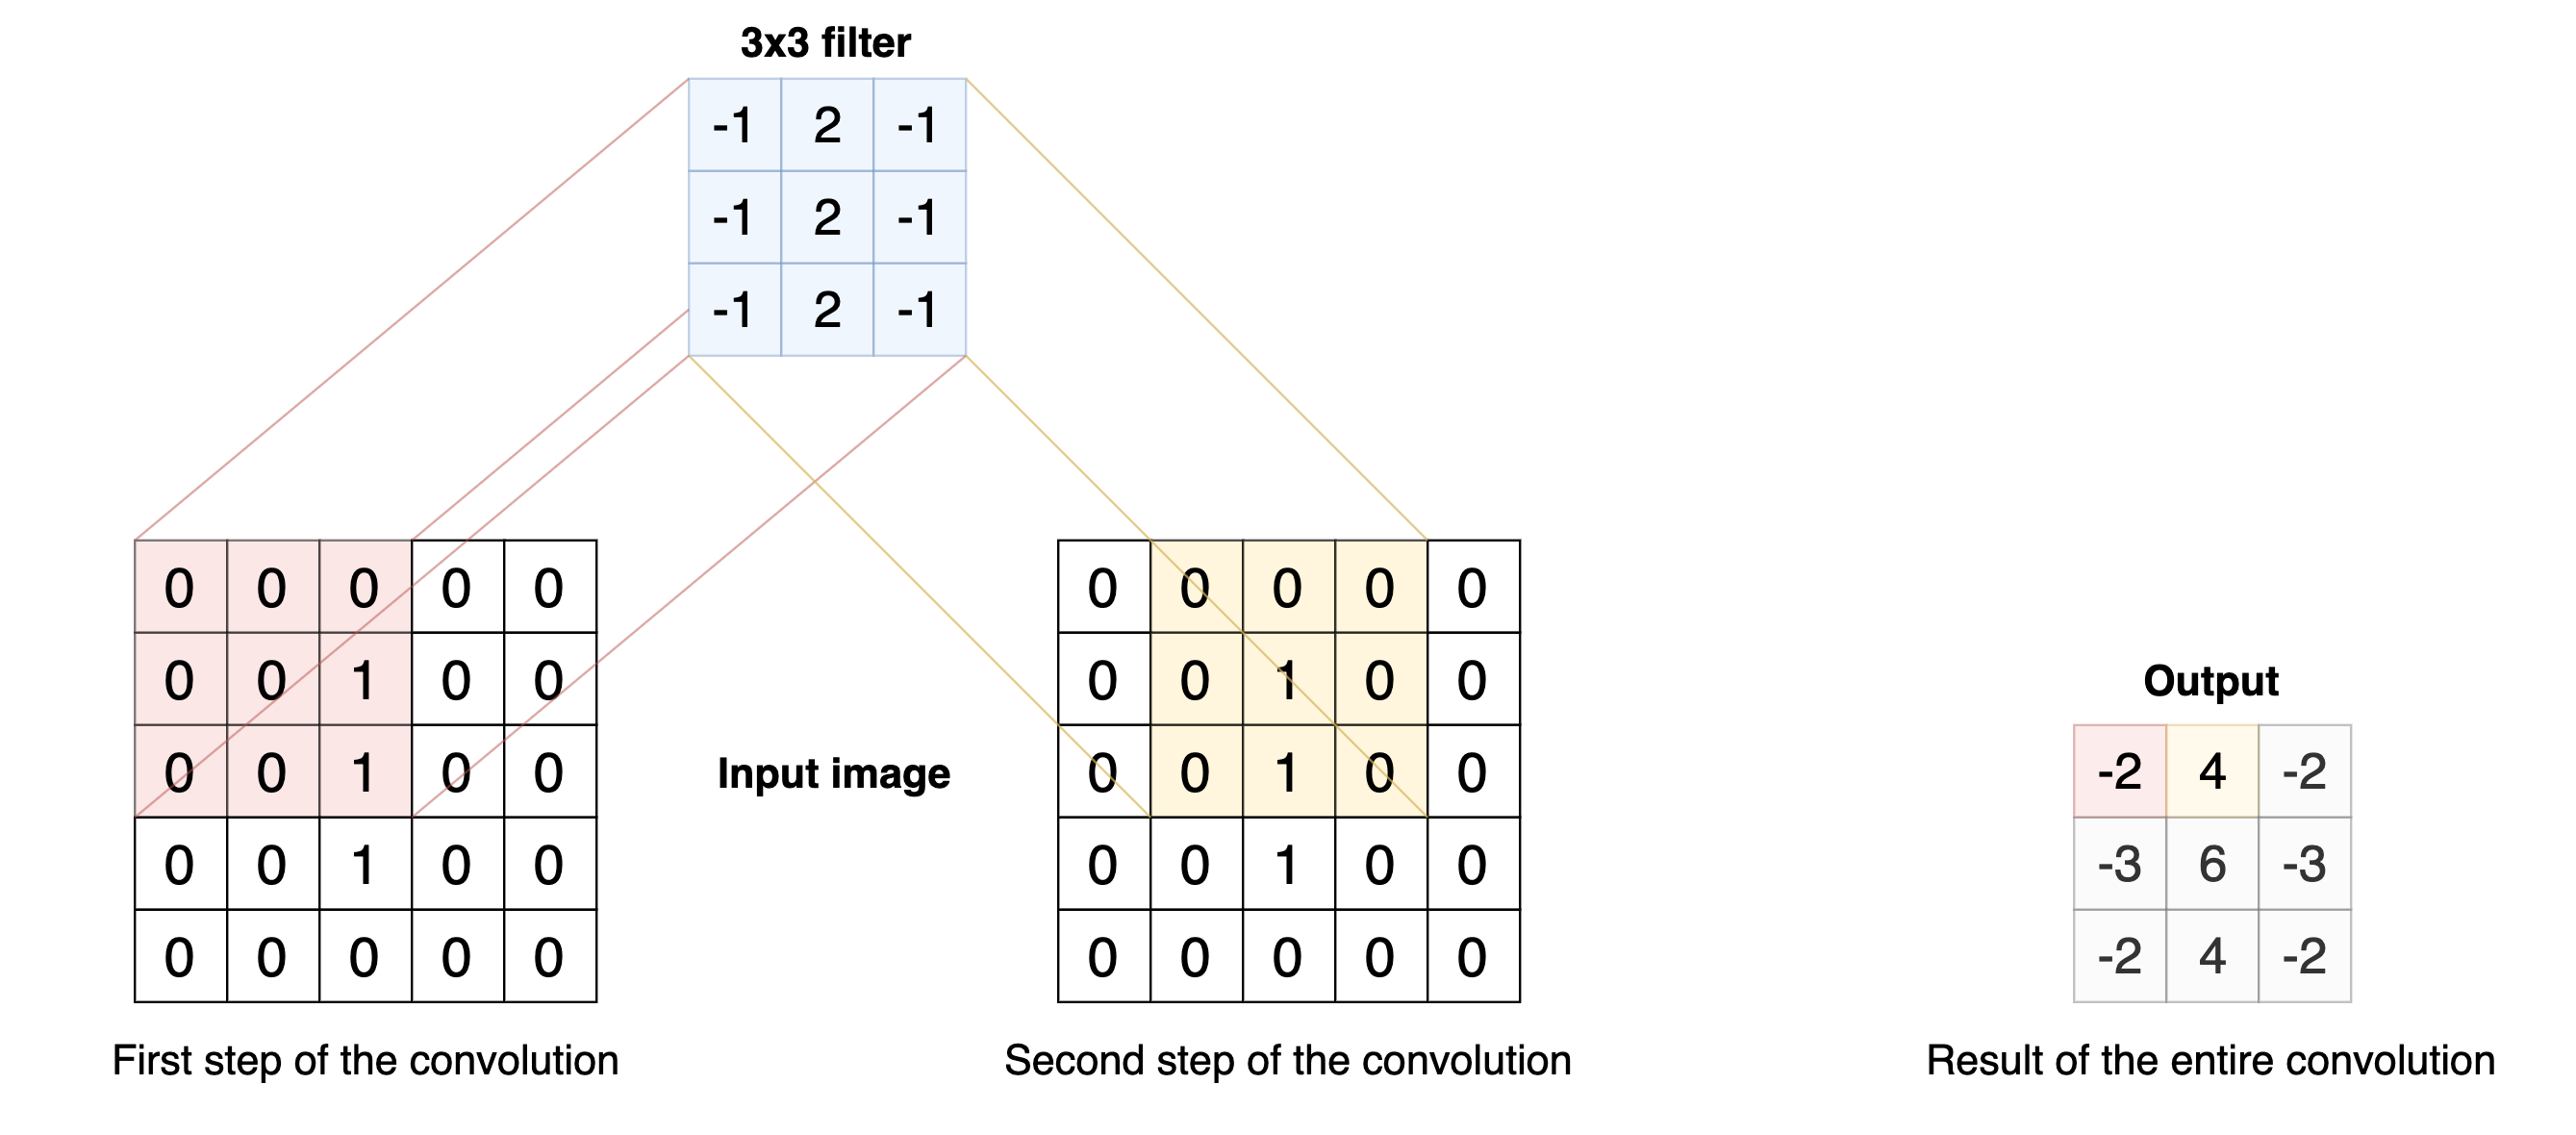
\includegraphics[width=1\textwidth, keepaspectratio=true]{./figures/convolution.png}
\caption{Convolutions - Basic convolution in a CNN}
\label{fig:convolution}
\end{figure}
\noindent Different parameters can change the way a convolution behaves. First of all, the previous example relied on a filter moving by respectively one cell to the right and to the bottom. In this case, the so-called "stride" is equal to 1. Other applications could rely on a bigger stride. Furthermore, the previous example reduced the output size of $3*3$ in proportion to the initial input size of $5*5$. To influence the output size, a padding can be added to the outside of the input image, usually filled with 0s. Three ways of padding images are commonly used as shown on Figure \ref{fig:convolution_padding}:
\begin{itemize}
	\item \textbf{Valid:} The input image is not padded. This means that the filter only goes through existing pixel values, which makes the output size smaller than the input size. 
	
	\item \textbf{Same:} The input image is padded in a way that makes the output size the same as the input size.
	
	\item \textbf{Full:} The input image is padded so that, in the first step of the convolution, only the bottom-right cell of the filter overlays the pixel values of the image, the rest overlaying padding cells. This makes the output size larger than the input size. 
\end{itemize}

\begin{figure}[!h]
\centering
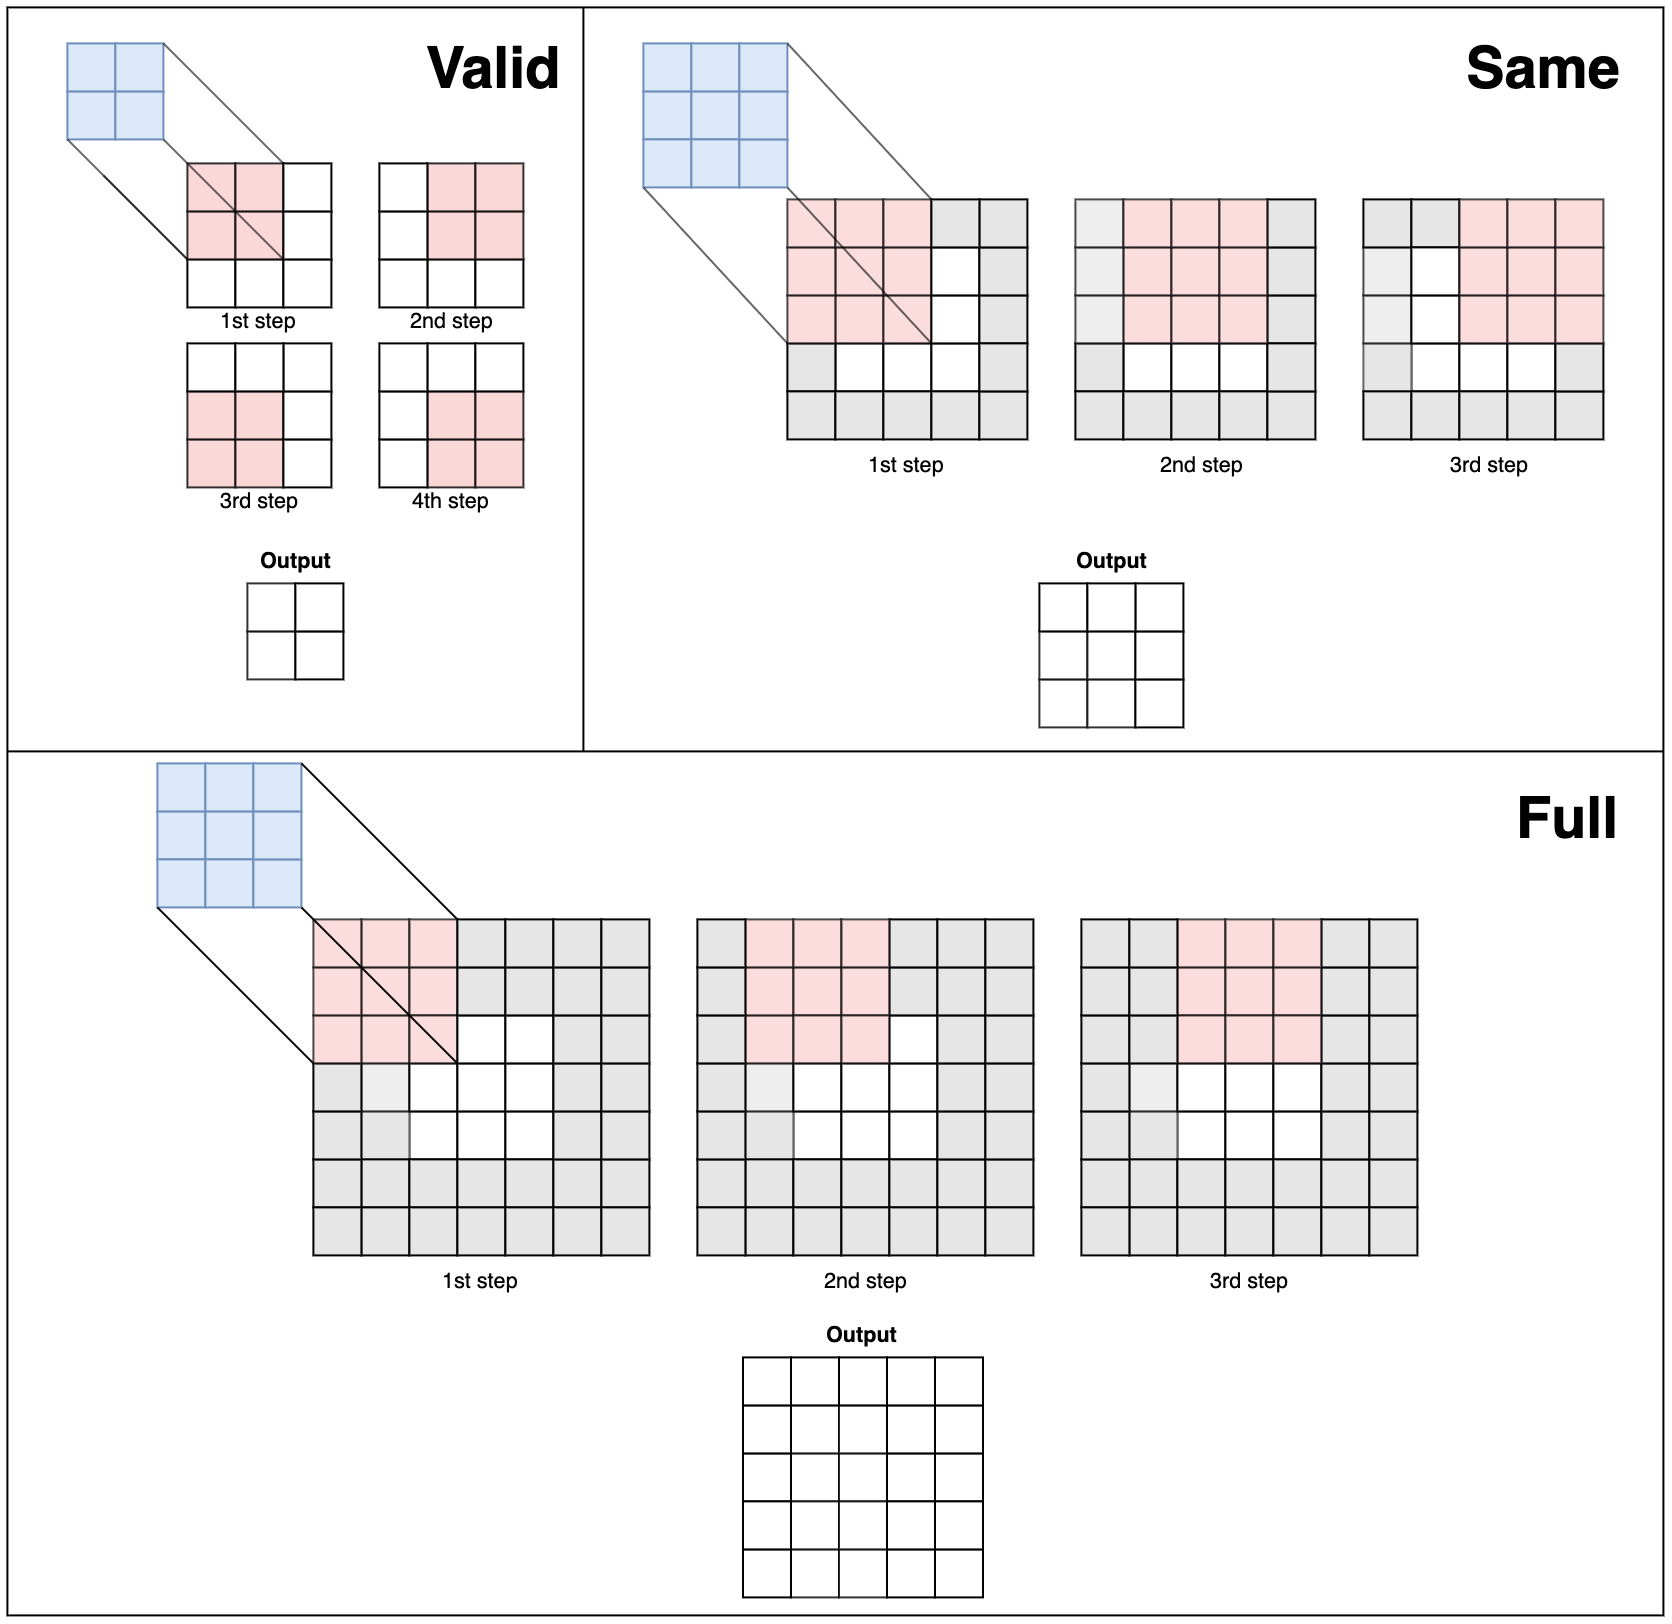
\includegraphics[width=1\textwidth, keepaspectratio=true]{./figures/convolution_padding.png}
\caption{Convolutions - Different padding methods}
\label{fig:convolution_padding}
\end{figure}



\section{Transfer learning}
\setlength{\marginparwidth}{3cm}\leavevmode \marginnote{\textbf{Jobin}}According to Jason Brownlee, "transfer learning is a machine learning method where a model developed for a task is reused as the starting point for a model on a second task"~\cite{30}. The model dedicated to the second task uses some or all parts of the first model (i.e. keeps the same weights and architecture or a part of them) and is then retrained on the data that is available for this task. The first model can either be implemented from scratch if enough data is available or downloaded from institutions that release large pretrained models for similar tasks. Transfer learning provides three major benefits~\cite{30}:
\begin{itemize}
\item Higher start: The initial skill (before refining the model) on the source model is higher than it otherwise would be.
\item Higher slope: The rate of skill improvement during training of the source model is steeper than it otherwise would be.
\item Higher asymptote: The converged skill of the trained model is better than it otherwise would be.
\end{itemize}
Nevertheless, "in general, it is not obvious that there will be a benefit to using transfer learning in the domain until after the model has been developed and evaluated"~\cite{30}.

